\documentclass{article}
\usepackage{graphicx}
\begin{document}

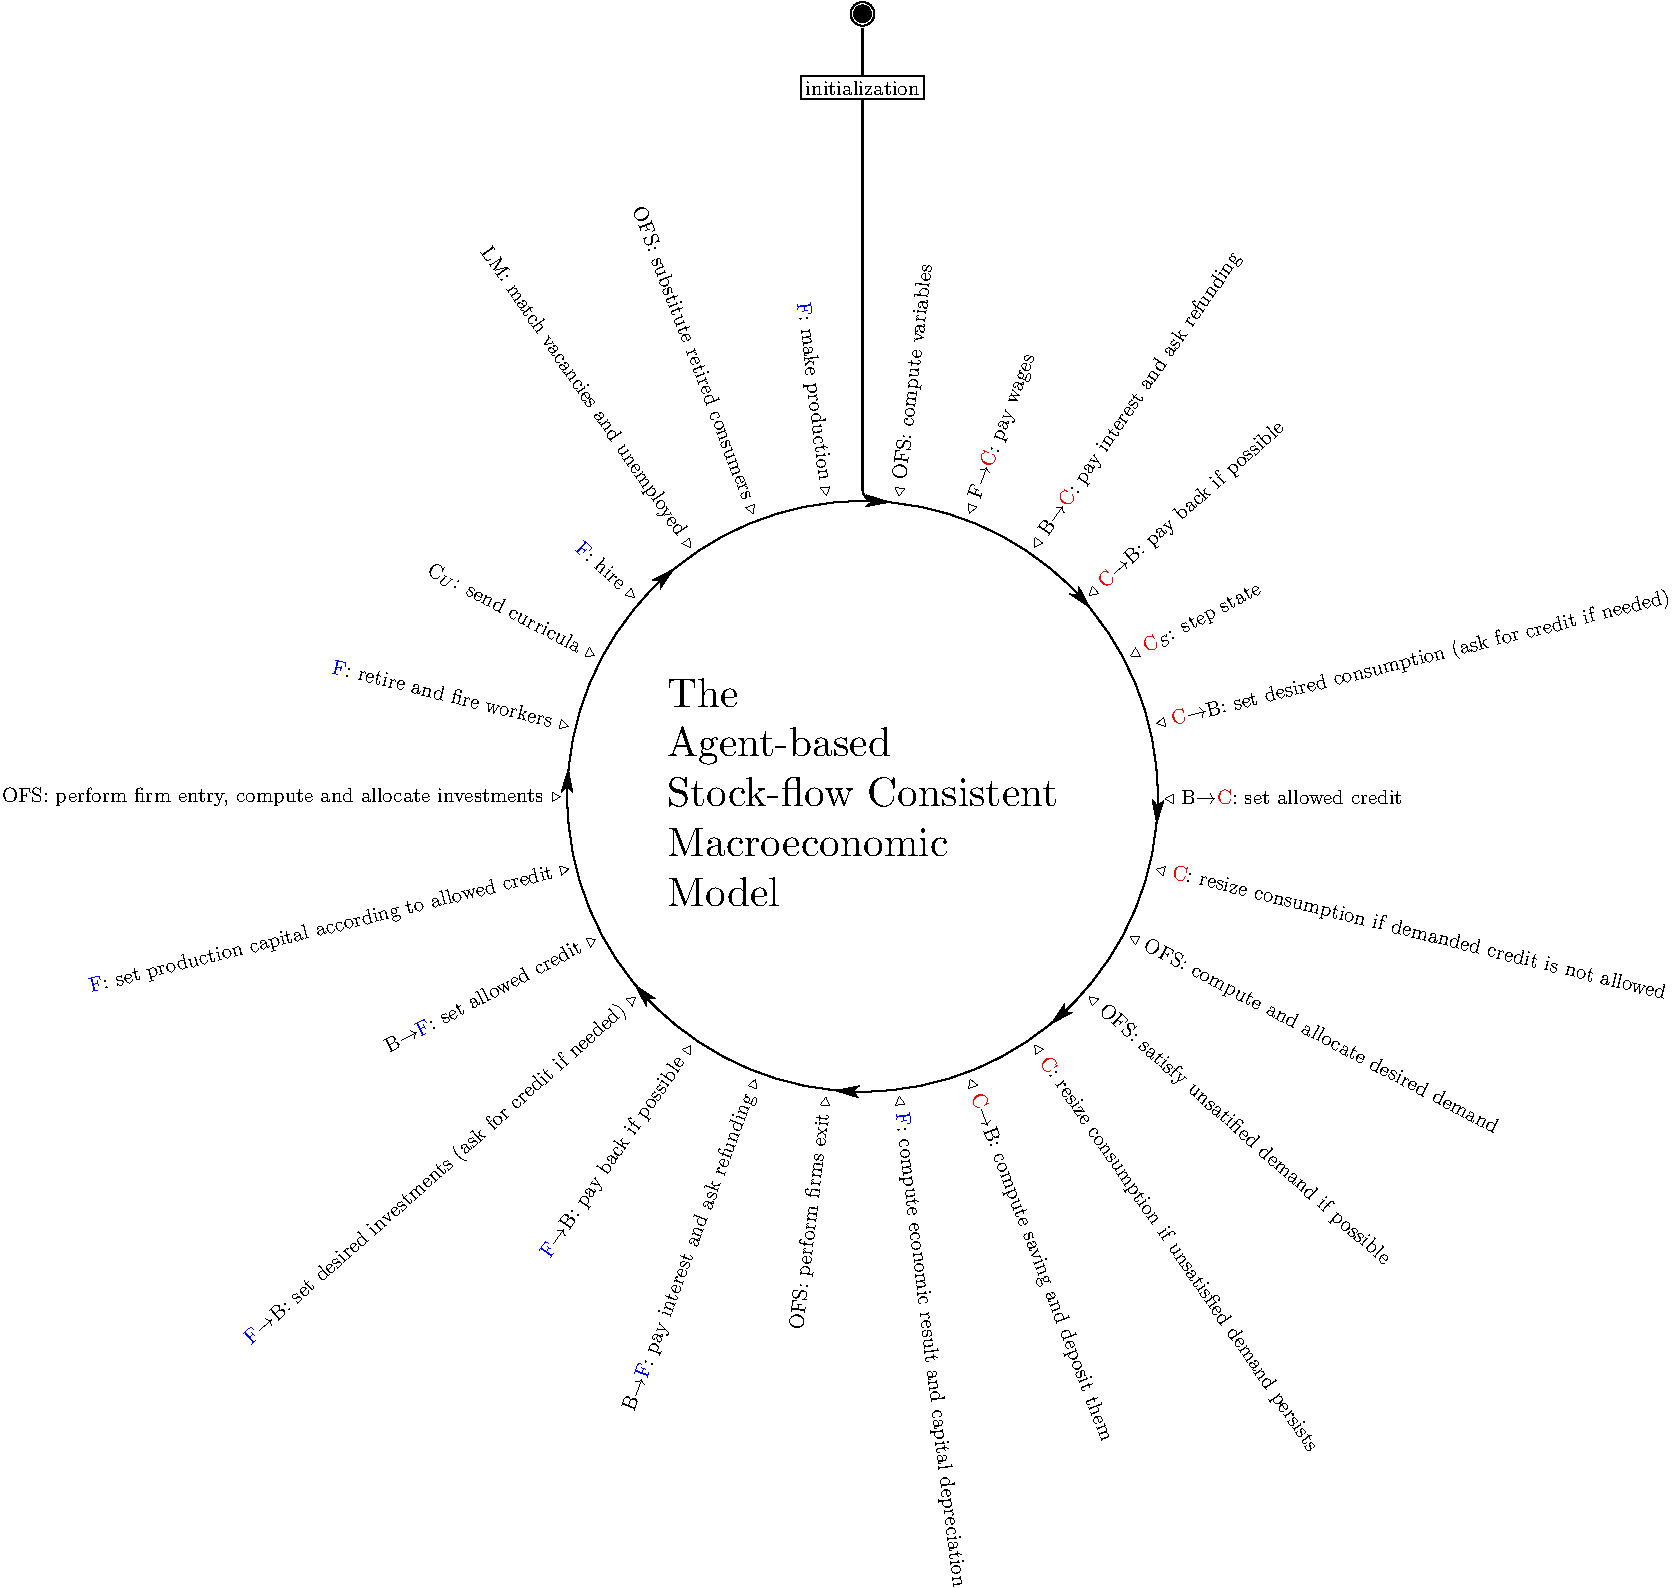
\includegraphics[scale=0.5]{visual.pdf}

\section{Bank-Consumer relationship}
The bank-consumer relationship progresses by the following steps

\begin{enumerate}
	\item banks account interests and ask for repayments to indebted consumers
	\item the consumer refund if possible
	\item the software performs a technical step by resetting some variables of the bank accounts
	\item consumers asks for new credit
	\item banks decide how much credit to allow
	\item consumers adjust desired consumption according to allowed credit. 
		
		Then, consumers try to gather the desired level of goods on the market. The effective level of consumption is established (it is less or equal to the desired consumption)
	\item consumers adjust bank accounts according to effective consumption.
\end{enumerate}
In the following we will present the dynamics of these events in some cases.


\subsection{Indebted Consumers}
\subsubsection*{Step 1: interests and ask for repayments}

Consumer can be customers of more banks.

First of all the banks account the interest rate.

Suppose that after accounting interest rate we have the following situation
\begin{verbatim}
bank 1 account =   10
bank 2 account = -150
bank 3 account =  -50
\end{verbatim}

The bank assumes that indebted consumers ask for the whole renewal of the debt:

\begin{verbatim}
bank 1 account =   10  demanded credit =    0
bank 2 account = -150  demanded credit = -150
bank 3 account =  -50  demanded credit =  -50
\end{verbatim}

Each bank with a negative account can ask for refunding. In this case the allowed credit is lower (in absolute value) to the demanded credit.
Suppose bank 2 and 3 as follow:

\begin{verbatim}
bank 1 account =   10  demanded credit =    0 allowed credit =    0
bank 2 account = -150  demanded credit = -150 allowed credit = -130 
bank 3 account =  -50  demanded credit =  -50 allowed credit =  -45
\end{verbatim}

In this example, the consumer needs 25 to satisfy banks requests.

\subsubsection*{step 2: refunding}
The consumer refund if she has enough income to refund and in any case refund an amount that guarantee him the subsistence consumption. Suppose for example that

\verb+disposableIncome=40+

and the subsistence consumption is 10.

The software first computes the resources available to refund. They are given by:

the sum of positive amounts in bank accounts plus the disposable income minus the subsistence consumption. In the example we have

\verb/resourceAvailableToRefund = 10 + 40 - 10 = 40/

They are enough to satisfy banks requests and 
the bank refund totally because her income allows both debt repayment and a consumption not less that the subsistence consumption. 
The new situation of the bank accounts in this situation is

\begin{verbatim}
bank 1 account =   10  demanded credit =    0 allowed credit =    0
bank 2 account = -130  demanded credit = -150 allowed credit = -130 
bank 3 account =  -45  demanded credit =  -50 allowed credit =  -45

disposableIncome = 15
\end{verbatim}


%If the income is not enough to refund and have the minimum consumption, the consumers makes a proposal to the bank by reducing the demand for credit. 

Suppose now that consumer's income is not 40 but 15:

\verb+disposableIncome = 15+

The resources available to refund (the sum of positive amounts in bank accounts plus the disposable income minus the subsistence consumption) are now

\verb/resourceAvailableToRefund = 10 + 15 - 10 = 15/

They are not enough to satisfy banks requests, so unpaid amounts are recorded and disposable income is set to allow the subsistence consumption:

\begin{verbatim}
bank 1: account =    0  demanded credit =    0 allowed credit =    0 unpaid =  0
bank 2: account = -135  demanded credit = -150 allowed credit = -130 unpaid =  5
bank 3: account =  -50  demanded credit =  -50 allowed credit =  -45 unpaid =  5

disposableIncome = 10
\end{verbatim}

\subsubsection*{Step 3: account resetting}
In this step, banks set the demanded and allowed credit are set to zero.

The new situation is

\begin{verbatim}
bank 1: account =    0  demanded credit =  0 allowed credit = 0 unpaid =  0
bank 2: account = -135  demanded credit =  0 allowed credit = 0 unpaid =  5
bank 3: account =  -50  demanded credit =  0 allowed credit = 0 unpaid =  5

disposableIncome = 10
\end{verbatim}




\subsubsection*{step 4: consumers set desired credit}
Now each consumer can asks for new credit. This can be done for two reasons: 1) to achieve a desired consumption higher than disposable income and 2) to pay unsatisfied lenders.

Suppose now that the consumer would like to consume 20.

She asks for additional financial resources both to finance consumption (10) and to pay back bank 2 and 3 (5+5).

The additional amount of 20 is asked to one bank. In particular, the bank with the best account (bank 1) is chosen. 

\begin{verbatim}
bank 1: account =    0  demanded credit = -20 allowed credit = 0 unpaid =  0
bank 2: account = -135  demanded credit =   0 allowed credit = 0 unpaid =  5
bank 3: account =  -50  demanded credit =   0 allowed credit = 0 unpaid =  5

disposableIncome = 10  desiredConsumption = 20
\end{verbatim}


\subsubsection*{Step 5: credit supply}

The bank decides how much credit to allow.

Suppose allowed credit is 18

\begin{verbatim}
bank 1: account =    0  demanded credit = -20 allowed credit = -18 unpaid =  0
bank 2: account = -135  demanded credit =   0 allowed credit =   0 unpaid =  5
bank 3: account =  -50  demanded credit =   0 allowed credit =   0 unpaid =  5

disposableIncome = 10  desiredConsumption = 20
\end{verbatim}

\subsubsection*{step 6: adjust consumption according to allowed credit}

In this step, the desired consumption is reduced by the difference between the demanded and the allowed credit. This reduction cannot make desired consumption be lower than the subsistence level.

In the example we have

\begin{verbatim}
bank 1: account =    0  demanded credit = -20 allowed credit = -18 unpaid =  0
bank 2: account = -135  demanded credit =   0 allowed credit =   0 unpaid =  5
bank 3: account =  -50  demanded credit =   0 allowed credit =   0 unpaid =  5

disposableIncome = 10  desiredConsumption = 18
\end{verbatim}

Now, the consumer goes in the goods market trying to satisfy her desires. It may happen that goods are in short supply. Suppose this is the case and she can buy 15 instead of 18. 

\subsubsection*{step 7: the consumer adjust bank accounts}

So the consumer can consume 15. 10 of them are payed by disposable income and 5 of them are borrowed from bank 1. 

Bank 1 is also willing to lend additional resources (18-5=13), so the consumer use it to satisfy bank 2 and 3 requests:

\begin{verbatim}
bank 1: account =  -15  demanded credit = -20 allowed credit = -18 unpaid =  0
bank 2: account = -130  demanded credit =   0 allowed credit =   0 unpaid =  0
bank 3: account =  -45  demanded credit =   0 allowed credit =   0 unpaid =  0

disposableIncome = 0  desiredConsumption = 18 effectiveConsumption = 15
\end{verbatim}



\section{Bank-Firm relationship}

The bank-firm relationship progresses by the following steps

\begin{enumerate}
	\item banks account interests and ask for repayments to indebted firms
	\item the firm refund if possible
	\item the software performs a technical step by resetting some variables of the bank accounts
	\item firms asks for new credit
	\item banks decide how much credit to allow
	\item firms adjust production capital and bank accounts
\end{enumerate}
In the following we will present the dynamics of these events in some cases.

\subsection{Bad condition}
\subsubsection*{Step 1: interests and ask for repayments}
Firm can be customers of more banks.

First of all banks account interests.

Suppose that after accounting interests we have the following situation
\begin{verbatim}
bank 1 account =   10
bank 2 account = -150
bank 3 account =  -50
\end{verbatim}

The bank assumes that Indebted firms ask for the whole renewal of the debt:

\begin{verbatim}
bank 1 account =   10  demanded credit =    0
bank 2 account = -150  demanded credit = -150
bank 3 account =  -50  demanded credit =  -50
\end{verbatim}

Each bank with a negative account can ask for refunding. In this case the allowed credit is lower (in absolute value) to the demanded credit.
Suppose bank 2 ask for refunding and bank 3 does not:

\begin{verbatim}
bank 1 account =   10  demanded credit =    0 allowed credit =    0
bank 2 account = -150  demanded credit = -150 allowed credit = -130 
bank 3 account =  -50  demanded credit =  -50 allowed credit =  -50
\end{verbatim}

In this example, the firm needs 20 to satisfy banks requests.

\subsubsection*{Step 2: refunding}

The possibility to refund depends on the resources available on banks and on the economic result. In our example, 10 is available in bank 1.

To go on with our example, let us assume that the economic result is \verb+-50+ i.e. the firm is suffering a loss.

The firm use 10 available in bank 1, but it is not enough to satisfy banks requests. Shortages are recorded as unpaid amounts.

The firm financial situation is represented as follows

\begin{verbatim}
bank 1: account =    0  demanded credit =    0 allowed credit =    0 unpaid =  0
bank 2: account = -140  demanded credit = -150 allowed credit = -130 unpaid = 10
bank 3: account =  -50  demanded credit =  -50 allowed credit =  -50 unpaid =  0

cashOnHand = -50
\end{verbatim}

\subsubsection*{Step 3: account resetting}
In this step, banks set the demanded and allowed credit are set to zero.

The new situation is

\begin{verbatim}
bank 1: account =    0  demanded credit =  0 allowed credit = 0 unpaid =  0
bank 2: account = -140  demanded credit =  0 allowed credit = 0 unpaid = 10
bank 3: account =  -50  demanded credit =  0 allowed credit = 0 unpaid =  0

cashOnHand = -50
\end{verbatim}



\subsubsection*{Step 4: set desired credit}

Now the firm can asks for new credit. This can be done for two reasons: 1) to finance new investments and 2) to pay unsatisfied lenders.

Suppose now that our firm do not invest, and ask for credit to pay unsatisfied lenders.

Credit in this step is asked to one of the banks, in particular to that with the best account.

In this example, the new asked credit is \verb/10+50=60/. The update situation is 

\begin{verbatim}
bank 1: account =    0  demanded credit = -60 allowed credit = 0 unpaid =  0
bank 2: account = -140  demanded credit =   0 allowed credit = 0 unpaid = 10
bank 3: account =  -50  demanded credit =   0 allowed credit = 0 unpaid =  0

cashOnHand = -50
\end{verbatim}






\subsubsection*{Step 5: credit supply}

The bank now decides the allowed credit.

The situation evolves differently according to the allowed amount.

Suppose first, the bank allows all the demanded credit. The situation is as follows

\begin{verbatim}
bank 1: account =    0  demanded credit = -60 allowed credit = -60 unpaid =  0
bank 2: account = -140  demanded credit =   0 allowed credit =   0 unpaid = 10
bank 3: account =  -50  demanded credit =   0 allowed credit =   0 unpaid =  0

cashOnHand = -50
\end{verbatim}

\subsubsection*{Step 6: the firm adjust bank accounts}

The resources made available by bank 1 are used and the situation evolve into the following

\begin{verbatim}
bank 1: account =  -60  demanded credit = -60 allowed credit = -60 unpaid =  0
bank 2: account = -130  demanded credit =   0 allowed credit =   0 unpaid =  0
bank 3: account =  -50  demanded credit =   0 allowed credit =   0 unpaid =  0

cashOnHand = 0
\end{verbatim}

\subsection{Good conditions}
	\subsubsection*{Step 1: interests and repayments}
	Suppose we start from the same conditions as in the bad cases.

	There are no differences in the evolution of this step, so that the situation at the end of this step is the same:
\begin{verbatim}
bank 1 account =   10  demanded credit =    0 allowed credit =    0
bank 2 account = -150  demanded credit = -150 allowed credit = -130 
bank 3 account =  -50  demanded credit =  -50 allowed credit =  -50
\end{verbatim}


	\subsubsection*{Step 2: refunding}
	Good condition here means that the firm realized a profit and thus has a positive cash on hand say

	\verb+cashOnHand = 50+

20 of them are used to refund the bank. So, now, the situation is 

\begin{verbatim}
bank 1: account =   10  demanded credit =    0 allowed credit =    0 unpaid =  0
bank 2: account = -130  demanded credit = -150 allowed credit = -130 unpaid =  0
bank 3: account =  -50  demanded credit =  -50 allowed credit =  -50 unpaid =  0

cashOnHand = 30
\end{verbatim}



	\subsubsection*{Step 3: account resetting}

\begin{verbatim}
bank 1: account =   10  demanded credit =    0 allowed credit =    0 unpaid =  0
bank 2: account = -130  demanded credit =    0 allowed credit =    0 unpaid =  0
bank 3: account =  -50  demanded credit =    0 allowed credit =    0 unpaid =  0

cashOnHand = 30
\end{verbatim}

	\subsubsection*{Step 4: set desired credit}
	Imagine now, the firm had a production capital equal to 100 before starting production. 
	
	Suppose production depreciates capital to 95.

	Furthermore, suppose the firm expects an increase of demand and wants to increase its production capital to 110.

	So, to bring production capital to the desired level 15 is needed.

	Checking financial resources available internally the firm conclude that it can achieve the objective without asking to banks. 

	Furthermore there is an inconsistency in firms bank accounts: the positive one should be used to reduce the negative ones. The software at this stage withdraws positive bank accounts and store them in the variable \verb+financialResourcesInBankAccounts+:

\begin{verbatim}
bank 1: account =    0  demanded credit =    0 allowed credit =    0 unpaid =  0
bank 2: account = -130  demanded credit =    0 allowed credit =    0 unpaid =  0
bank 3: account =  -50  demanded credit =    0 allowed credit =    0 unpaid =  0

cashOnHand = 30 financialResourcesInBankAccounts = 10
\end{verbatim}

	\subsubsection*{Step 5: credit supply}
In this step no change is performed because credit was not asked.

	\subsubsection*{Step 6: adjust production capital and banks accounts}

	Production capital is adjusted by using internal financial resources. 

	So, after this step we have

	\verb+productionCapital=110+

	\verb/cashOnHand + financialResourcesInBankAccounts = 25/

	finally, the residual internal refunds are used to improve the worst bank account:

\begin{verbatim}
bank 1: account =    0  demanded credit =    0 allowed credit =    0 unpaid =  0
bank 2: account = -105  demanded credit =    0 allowed credit =    0 unpaid =  0
bank 3: account =  -50  demanded credit =    0 allowed credit =    0 unpaid =  0

cashOnHand = 0 financialResourcesInBankAccounts = 0
\end{verbatim}





\end{document}
